% IEEE conference manuscript for the PINN-EV-Battery project.
% Compile on Overleaf with pdfLaTeX. Keep this file beside figures/.
% IMPORTANT: fill the result macros only from the complete three-seed run.
\documentclass[conference]{IEEEtran}
\IEEEoverridecommandlockouts

% Packages from the official IEEE conference template.
\usepackage{cite}
\usepackage{amsmath,amssymb,amsfonts}
\usepackage{iftex}
% Tectonic uses XeTeX for local previews.  Give headings a real bold Times
% face there while preserving the standard IEEEtran body typography.
\ifXeTeX
  \usepackage{fontspec}
  \newfontfamily\headingfont{TeXGyreTermesX-Regular.otf}[
    BoldFont=TeXGyreTermesX-Bold.otf]
\else
  \newcommand{\headingfont}{\rmfamily}
\fi
\usepackage{algorithmic}
\usepackage{graphicx}
\usepackage{stfloats} % enables bottom placement of full-width IEEE figures
\usepackage{textcomp}
\usepackage{xcolor}

% Additional packages required by this manuscript's tables and units.
\usepackage{booktabs}
\usepackage{multirow}
\usepackage{array}
\usepackage{siunitx}
\usepackage{url}
\usepackage{balance}

% Clear heading hierarchy requested for the conference manuscript:
% sections are 12 pt bold, while subsections remain 10 pt bold.
% Use battery_pinn_ieee_conference_strict.tex if a venue requires the
% untouched IEEEtran heading definitions.
\makeatletter
\def\section{\@startsection{section}{1}{\z@}{1.5ex plus 1.5ex minus 0.5ex}%
{0.7ex plus 1ex minus 0ex}{\normalfont\headingfont\large\centering\bfseries}}
\def\subsection{\@startsection{subsection}{2}{\z@}{1.5ex plus 1.5ex minus 0.5ex}%
{0.7ex plus .5ex minus 0ex}{\normalfont\headingfont\normalsize\bfseries}}
\def\subsubsection{\@startsection{subsubsection}{3}{\parindent}{0ex plus 0.1ex minus 0.1ex}%
{0ex}{\normalfont\headingfont\normalsize\bfseries\itshape}}
\makeatother

\def\BibTeX{{\rm B\kern-.05em{\sc i\kern-.025em b}\kern-.08em
    T\kern-.1667em\lower.7ex\hbox{E}\kern-.125emX}}

\graphicspath{{figures/}}
\sisetup{detect-all,table-number-alignment=center}
\newcommand{\modelname}{PC-MP-PINN}

% Set \resultsavailabletrue only after inserting values from
% results/paper_metrics_summary.csv and variation_gap_vs_previous.csv.
\newif\ifresultsavailable
\resultsavailablefalse
\newcommand{\pending}{\textit{pending}}
\newcommand{\DataC}{\pending}
\newcommand{\PriorC}{\pending}
\newcommand{\ProposedC}{\pending}
\newcommand{\DataT}{\pending}
\newcommand{\PriorT}{\pending}
\newcommand{\ProposedT}{\pending}
\newcommand{\DataStress}{\pending}
\newcommand{\PriorStress}{\pending}
\newcommand{\ProposedStress}{\pending}
\newcommand{\DataMass}{\pending}
\newcommand{\PriorMass}{\pending}
\newcommand{\ProposedMass}{\pending}
\newcommand{\DataSpeed}{\pending}
\newcommand{\PriorSpeed}{\pending}
\newcommand{\ProposedSpeed}{\pending}

\title{{\headingfont\bfseries A Physics-Consistent Electrochemical--Thermal PINN with Concentration-Coupled Particle Stress for Lithium-Ion Battery Surrogate Modeling}}

\author{
\IEEEauthorblockN{1\textsuperscript{st} Ms. Sasikala C,
2\textsuperscript{nd} Naresh V,
3\textsuperscript{rd} Mohamed Shaheel A,
4\textsuperscript{th} Kishore J,
5\textsuperscript{th} Kishore P. S.}
\IEEEauthorblockA{\textit{Department of Computer Science and Engineering} \\
\textit{KPR Institute of Engineering and Technology}\\
Coimbatore, Tamil Nadu, India}
}

\begin{document}
\maketitle

\begin{abstract}
A structured comparison of ten recent physics-informed battery studies shows strong progress in electrochemical surrogates, thermal prediction, parameter estimation, and degradation-aware health modeling, while also showing that multiphysics coupling alone is not a defensible novelty claim. This paper therefore studies a narrower gap: a battery surrogate can remain physically ambiguous when mechanical outputs are learned independently of the electrochemical state that causes them. We present a physics-consistent multiphysics PINN (\modelname) for constant-current discharge of a lithium-ion cell. The model predicts negative-particle lithium concentration and lumped cell temperature from radius, time, C-rate, and ambient temperature. Solid diffusion, center symmetry, surface flux, and energy balance enter the training loss; radial and tangential stresses are obtained from predicted concentration through an analytical spherical-particle elasticity operator instead of independent stress heads. PyBaMM SPMe simulations with Chen2020 parameters provide reference trajectories. A condition-wise protocol compares data-only, independently learned-stress PINN, and proposed variants across three label budgets and three seeds. Nine metrics cover field accuracy, peak stress, mass conservation, cross-field consistency, and inference speed. The scope is discharge-state surrogate modeling; experimental validation, degradation, state of health, and remaining useful life are not claimed without the corresponding data.
\end{abstract}

\begin{IEEEkeywords}
physics-informed neural network, lithium-ion battery, SPMe, thermal model, diffusion-induced stress, multiphysics surrogate, sparse data
\end{IEEEkeywords}

\section{Introduction}
Lithium-ion battery management requires rapid estimates of quantities that cannot be measured directly, including concentration gradients inside active-material particles and the stresses induced by repeated lithium insertion and removal. High-fidelity electrochemical models describe these states through coupled differential equations, but their repeated numerical solution can be expensive for optimization, uncertainty analysis, and embedded control. The Doyle--Fuller--Newman formulation established a foundational porous-electrode description of galvanostatic lithium-cell behavior \cite{doyle1993dfn}. Reduced-order electrochemical models such as the single-particle model with electrolyte dynamics (SPMe) retain key transport behavior at lower cost \cite{marquis2019spme,richardson2020gspm,planella2022continuum}. Physics-informed neural networks provide another reduction mechanism: a neural approximation is trained simultaneously from available state labels and residuals of the governing equations \cite{raissi2019pinn}.

Battery PINN studies now cover electrochemical parameter identification, thermal-state prediction, SPM and pseudo-two-dimensional (P2D) surrogates, and health estimation \cite{hassanaly2024part1,hassanaly2024part2,wang2023temperature,wang2024parameter}. Therefore, a claim that electrochemical, thermal, and mechanical quantities merely appear in one network is insufficient. In particular, Wei \emph{et al.} already introduced an electrochemical--thermal--mechanical aging-informed framework for state-of-health estimation that includes solid-electrolyte-interphase growth, lithium plating, and particle fracture \cite{wei2026etm}. The scientific question must be more specific.

The weakness addressed here is cross-field consistency. In a prior formulation, radial stress and tangential stress were direct neural outputs. A mechanical-equilibrium residual constrained those outputs, but it did not uniquely force them to arise from the predicted lithium concentration. A network could therefore fit plausible stress labels while drifting from the electrochemical state. We replace those stress heads with the Cheng--Verbrugge spherical-particle stress operator \cite{cheng2009stress}. This creates an explicit causal chain from concentration to stress.

The contributions are:
\begin{enumerate}
    \item a parameterized PINN for negative-particle concentration and lumped temperature over C-rate and ambient-temperature conditions;
    \item a deterministic concentration-to-stress construction that removes independent mechanical degrees of freedom;
    \item leakage-resistant evaluation using condition-wise train, validation, and test sets, with checkpoint selection based only on validation data;
    \item a controlled comparison across three formulations, three label budgets, and three random seeds using field, peak, conservation, consistency, and inference-efficiency metrics; and
    \item a precise statement of scope separating single-discharge mechanics from cycle-dependent degradation and health estimation.
\end{enumerate}

\section{Related Work and Research Gap}
\subsection{Physics-Informed Battery Surrogates}
Raissi \emph{et al.} established the modern PINN framework by combining observation loss with residuals of differential equations \cite{raissi2019pinn}. In battery modeling, Hassanaly \emph{et al.} developed SPM and P2D PINN surrogates for parameter inference, showing both the promise of low-data training and the importance of conservation regularization and hierarchical training \cite{hassanaly2024part1,hassanaly2024part2}. Jingrong Wang \emph{et al.} used multiple PINN branches to identify electrochemical parameters across operating conditions \cite{wang2024parameter}. Zhuang \emph{et al.} later benchmarked conventional PINNs and a DeepONet-based architecture for SPM surrogate modeling \cite{zhuang2026spm}. These works motivate electrochemical residuals and careful low-data evaluation, but particle stress is outside their main prediction target.

\subsection{Recent 2024--2026 Context}
Recent work has broadened physics-informed battery learning beyond PDE surrogates. Fu \emph{et al.} embedded an equivalent-circuit model in a recurrent network for spacecraft-battery modeling, while Dang \emph{et al.} imposed differential-equation structure for state-of-charge estimation \cite{fu2024spacecraft,dang2024soc}. Jiang \emph{et al.} combined low- and high-fidelity information for battery-pack heat-map prediction \cite{jiang2025heatmap}. Recent health studies use physics-informed features, transfer learning, small-sample degradation dynamics, and electrochemical--thermal--mechanical side-reaction priors \cite{ye2024soh,tian2025generic,xiong2025diagnostics,chen2025smallsample,luo2025hybrid}. These studies reinforce the need to state whether physics enters through equations, architecture, features, or regularization; the present work specifically enforces concentration--stress consistency in a discharge surrogate.

\subsection{Thermal and Mechanical Coupling}
Yuchen Wang \emph{et al.} embedded electrical, heat-generation, and thermal relations in a recurrent battery-informed model for life-cycle temperature prediction \cite{wang2023temperature}. Lyu \emph{et al.} coupled electrochemical, thermal, and particle-stress models in a digital twin, directly demonstrating that the presence of all three domains is not itself new \cite{lyu2024digitaltwin}. Their objectives differ from the present sparse-label comparison of independently predicted versus concentration-derived stress. The analytical mechanics used here follows spherical-particle stress models \cite{cheng2009stress,christensen2006fracture}. Insertion-driven volume change couples stress with transport, reaction, deformation, and fracture \cite{xu2016electrochemomechanics}. Uniform concentration gives zero diffusion-induced stress; nonuniformity generates radial and tangential stress.

\subsection{Why Mechanics Is Retained}
Replacing mechanics with degradation is not necessary for the present research question. Mechanics describes an instantaneous consequence of a concentration gradient during one discharge. Degradation describes irreversible evolution over many cycles and requires cycle index, capacity or state-of-health labels, and mechanisms such as SEI growth, lithium plating, active-material loss, or crack propagation. Both can coexist in a future model, but adding degradation changes the target from a discharge surrogate to an aging model. The current dataset does not support that change. Table~\ref{tab:gap} positions the proposed work without claiming that multiphysics coupling itself is unprecedented.

\begin{table*}[t]
\centering
\caption{Positioning Against Ten Recent Physics-Informed Battery Studies}
\label{tab:gap}
\scriptsize
\renewcommand{\arraystretch}{1.08}
\setlength{\tabcolsep}{2.5pt}
\begin{tabular}{>{\raggedright\arraybackslash}p{2.55cm}>{\raggedright\arraybackslash}p{2.55cm}>{\raggedright\arraybackslash}p{3.0cm}>{\raggedright\arraybackslash}p{1.65cm}>{\raggedright\arraybackslash}p{2.35cm}>{\raggedright\arraybackslash}p{3.7cm}}
\toprule
Study & Main task & Physics represented & Thermal state & Mechanics / aging & Key distinction from this work \\
\midrule
Hassanaly \emph{et al.}, Part I (2024) \cite{hassanaly2024part1} & SPM surrogate; parameter inference & Diffusion PINN; multi-fidelity hierarchy & \textbf{None} & \textbf{None} & \textbf{No thermal/stress fields}; closest electrochemical surrogate \\
\addlinespace[1pt]
Hassanaly \emph{et al.}, Part II (2024) \cite{hassanaly2024part2} & P2D surrogate; Bayesian inference & Electrochemical transport; conservation regularization & \textbf{None} & \textbf{None} & \textbf{Higher electrochemical fidelity}; no particle-stress test \\
\addlinespace[1pt]
Y. Wang \emph{et al.} (2023) \cite{wang2023temperature} & Life-cycle temperature prediction & Electrical and heat-generation models & \textbf{Cell temperature} & Aging through learned parameters & \textbf{Thermal sequence model}; no radial concentration/stress fields \\
\addlinespace[1pt]
J. Wang \emph{et al.} (2024) \cite{wang2024parameter} & Electrochemical parameter identification & Parallel PINN branches; electrochemical model & Operating effect only & \textbf{None} & \textbf{Parameter inference}; no concentration--stress consistency test \\
\addlinespace[1pt]
Lyu \emph{et al.} (2024) \cite{lyu2024digitaltwin} & Lithium-ion battery digital twin & Electrochemical--thermal--mechanical coupling & \textbf{Yes} & \textbf{Particle stress} & \textbf{Already combines E--T--M}; no sparse-label stress ablation \\
\addlinespace[1pt]
Fu \emph{et al.} (2024) \cite{fu2024spacecraft} & Spacecraft-battery model; health diagnosis & Equivalent-circuit physics; recurrent learning & No spatial field & Health diagnosis & \textbf{System-level model}; no particle concentration/stress fields \\
\addlinespace[1pt]
Dang \emph{et al.} (2024) \cite{dang2024soc} & State-of-charge estimation & Differential-equation-informed network & \textbf{None} & \textbf{None} & \textbf{SOC target}; no internal multiphysics fields \\
\addlinespace[1pt]
Jiang \emph{et al.} (2025) \cite{jiang2025heatmap} & Battery-pack heat-map prediction & Multi-fidelity CNN; heat-transfer constraints & \textbf{Pack heat map} & \textbf{None} & \textbf{Pack-scale thermal field}; no particle stress \\
\addlinespace[1pt]
Wei \emph{et al.} (2026) \cite{wei2026etm} & State-of-health estimation & Electrochemical--thermal--mechanical aging PINN & \textbf{Yes} & \textbf{SEI, plating, fracture} & \textbf{Cycling/health model}; broader target and data needs \\
\addlinespace[1pt]
Zhuang \emph{et al.} (2026) \cite{zhuang2026spm} & SPM surrogate under varying currents & PINNs; Fourier-enhanced DeepONet & \textbf{None} & \textbf{None} & \textbf{Dynamic-current electrochemistry}; no thermal/mechanical output \\
\bottomrule
\end{tabular}
\end{table*}

\section{Governing Physics}
\subsection{Solid-Phase Lithium Diffusion}
The negative active-material particle is treated as a sphere of radius $R_p$ with radial coordinate $r$. Under spherical symmetry and constant solid diffusivity $D_s$, lithium concentration $c_s(r,t)$ satisfies Fickian diffusion:
\begin{equation}
\frac{\partial c_s}{\partial t}=D_s\left(\frac{\partial^2 c_s}{\partial r^2}+\frac{2}{r}\frac{\partial c_s}{\partial r}\right).
\label{eq:diffusion}
\end{equation}
The center-symmetry, interfacial-flux, and initial conditions are
\begin{align}
\left.\frac{\partial c_s}{\partial r}\right|_{r=0}&=0, \\
-D_s\left.\frac{\partial c_s}{\partial r}\right|_{r=R_p}&=\frac{j_n(t)}{F},
\label{eq:flux}\\
c_s(r,0)&=c_{s,0},
\end{align}
where $j_n$ is the negative-electrode interfacial current density and $F$ is Faraday's constant. The SPMe reference is generated in PyBaMM, an open-source battery modeling framework \cite{sulzer2021pybamm}, using the Chen2020 LG M50 parameterization \cite{chen2020parameterization}.

\subsection{Lumped Thermal Balance}
The reference simulation uses a volume-averaged cell temperature. Battery energy balances connect heat generation and cooling \cite{bernardi1985energy}. The compatible lumped energy balance is
\begin{equation}
\rho_{\mathrm{eff}}c_{p,\mathrm{eff}}\frac{dT}{dt}
=q_{\mathrm{gen}}(t)-\frac{hA_{\mathrm{cool}}}{V_{\mathrm{cell}}}(T-T_{\mathrm{amb}}),
\label{eq:thermal}
\end{equation}
where $q_{\mathrm{gen}}$ is volumetric heat generation, $h$ is the heat-transfer coefficient, and $A_{\mathrm{cool}}/V_{\mathrm{cell}}$ is the cooling-area-to-volume ratio. Since $T$ is lumped, the proposed temperature network does not receive $r$; allowing a radial input would introduce a degree of freedom that the assumed physics cannot identify.

\subsection{Diffusion-Induced Particle Stress}
Let
\begin{equation}
\mathcal{A}(r,t)=\frac{1}{r^3}\int_{0}^{r}c_s(s,t)s^2\,ds,
\quad
K=\frac{\Omega E}{3(1-\nu)},
\label{eq:A}
\end{equation}
where $\Omega$ is partial molar volume, $E$ is Young's modulus, and $\nu$ is Poisson's ratio. The radial and tangential stresses are computed as \cite{cheng2009stress}
\begin{align}
\sigma_r(r,t)&=2K[\mathcal{A}(R_p,t)-\mathcal{A}(r,t)],
\label{eq:sr}\\
\sigma_\theta(r,t)&=K[2\mathcal{A}(R_p,t)+\mathcal{A}(r,t)-c_s(r,t)].
\label{eq:st}
\end{align}
Equations~\eqref{eq:A}--\eqref{eq:st} are applied to the predicted concentration. The stress field is therefore mechanically interpretable but remains an analytical, linear-elastic estimate; it is not an experimental stress measurement or a crack-evolution model.

\section{Proposed Physics-Consistent PINN}
\subsection{Architecture and Hard Constraints}
Figure~\ref{fig:architecture} shows the model. Inputs are normalized radius $\bar r=r/R_p$, normalized physical time $\tau=t/t_{\mathrm{ref}}$, C-rate $C$, and ambient temperature $T_{\mathrm{amb}}$. The fixed scale $t_{\mathrm{ref}}=7200$~s is used for every condition. This avoids normalizing by each trajectory's final discharge time, which would reveal future information at inference.

Two fully connected subnetworks use four hidden layers of 96 neurons with hyperbolic-tangent activations. The concentration head receives $(\bar r,\tau,C,T_{\mathrm{amb}})$; the lumped temperature head receives $(\tau,C,T_{\mathrm{amb}})$. Initial conditions are imposed by the output transformations
\begin{align}
\widehat{c}_s(\bar r,\tau)&=c_{s,0}+\tau\,\mathcal{N}_c(\bar r,\tau,C,T_{\mathrm{amb}}),
\label{eq:hardc}\\
\widehat{T}(\tau)&=T_{\mathrm{amb}}+\Delta T_{\mathrm{scale}}\tau\,
\mathcal{N}_T(\tau,C,T_{\mathrm{amb}}),
\label{eq:hardt}
\end{align}
with $\Delta T_{\mathrm{scale}}=50$~K. Stress is calculated from $\widehat{c}_s$ using Eqs.~\eqref{eq:A}--\eqref{eq:st} on the evaluation grid.

\begin{figure*}[t]
\centering
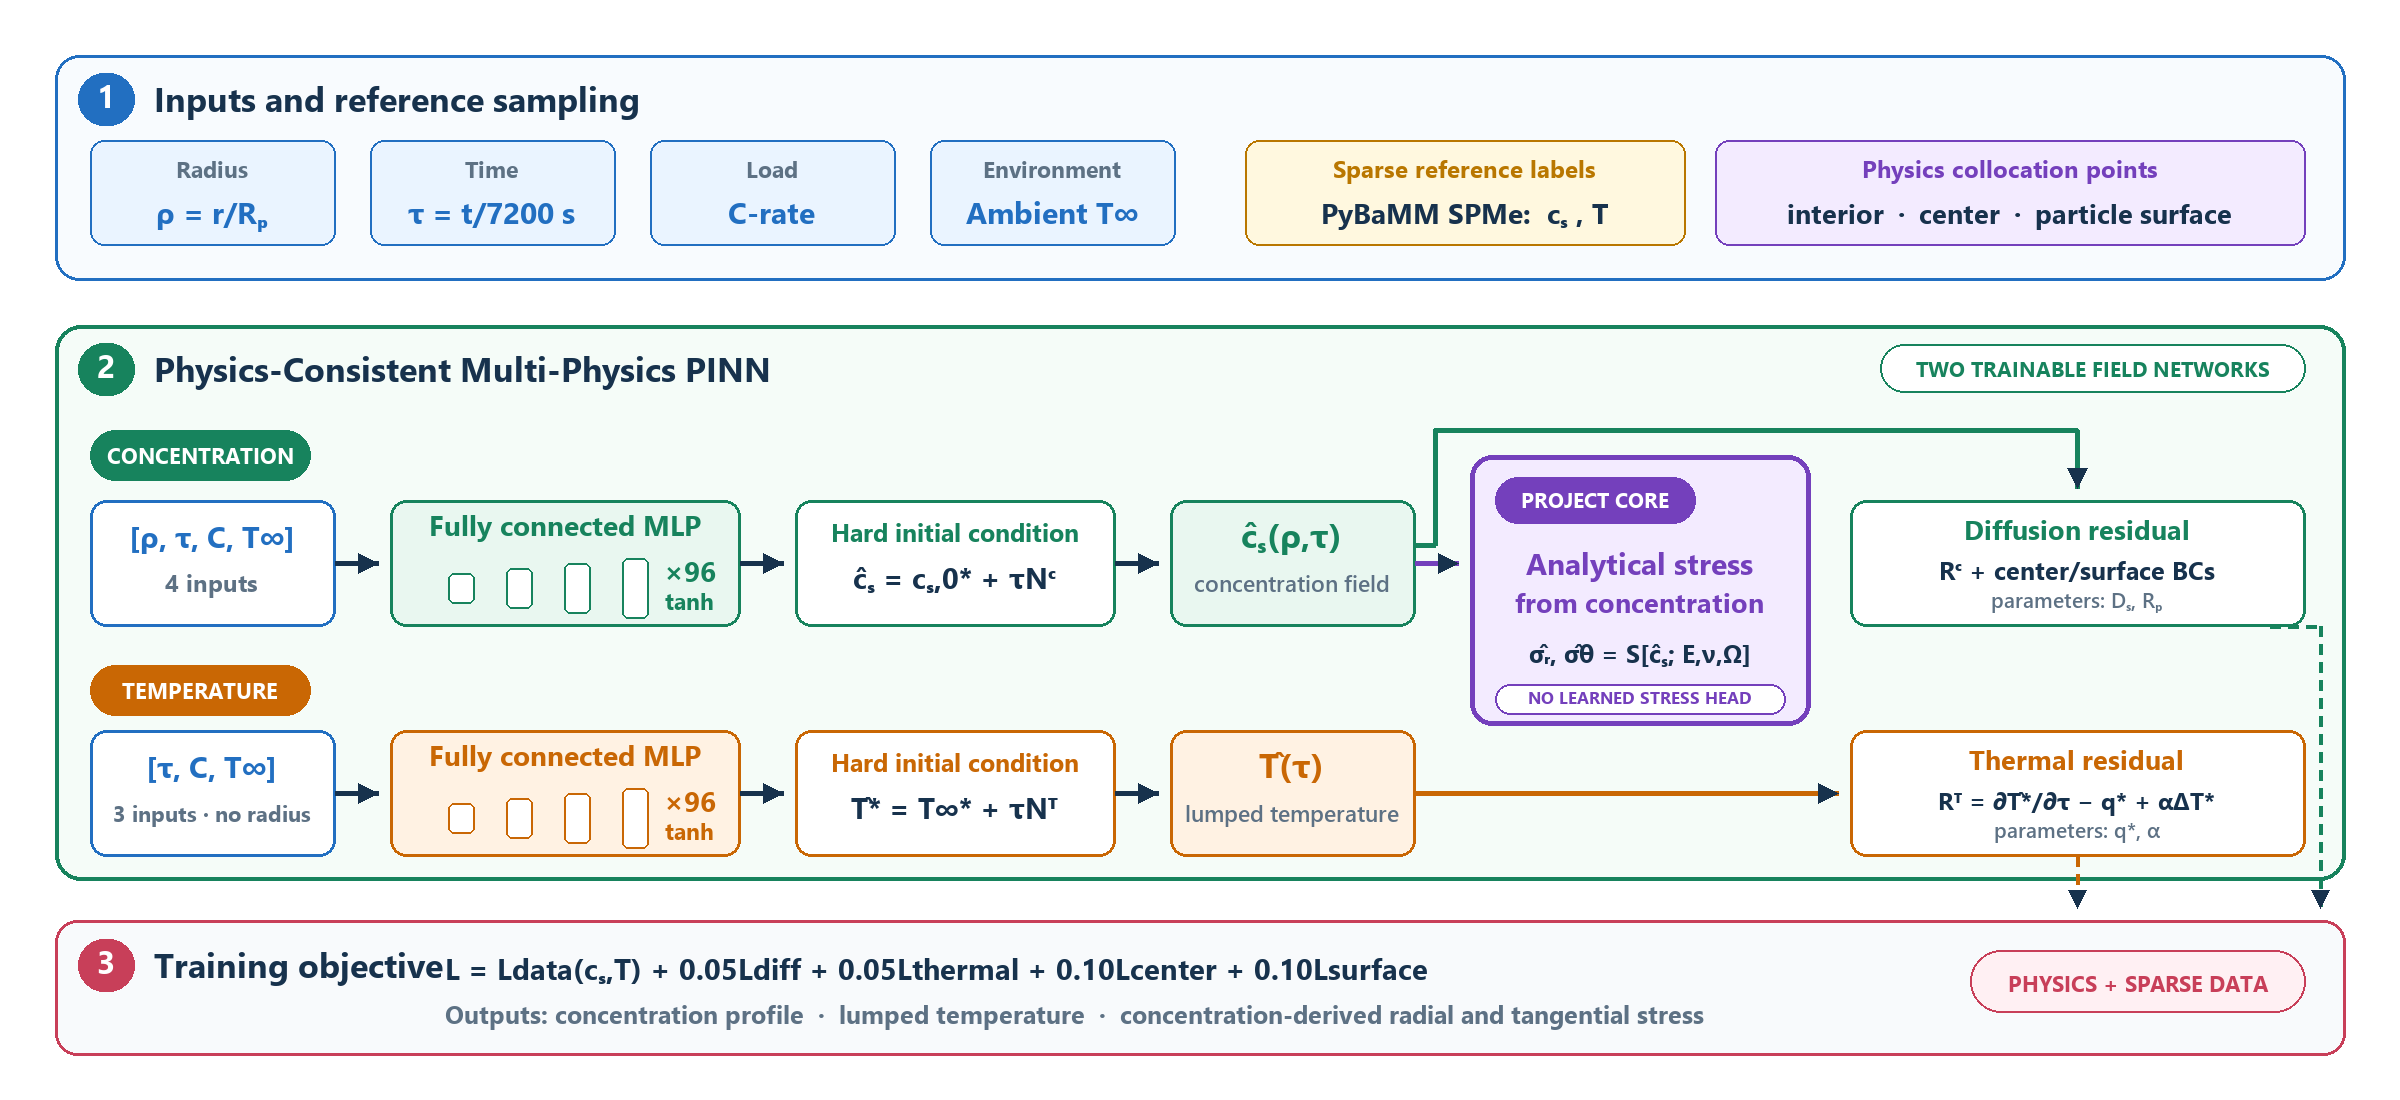
\includegraphics[width=\textwidth]{pinn_architecture.png}
\caption{Proposed \modelname{} architecture. The temperature branch matches the lumped thermal assumption, while stress is an analytical function of predicted concentration.}
\label{fig:architecture}
\end{figure*}

\subsection{Physics Residuals}
Automatic differentiation provides derivatives of neural outputs. In dimensionless coordinates, the diffusion residual is
\begin{equation}
\mathcal{R}_{c}=\frac{\partial \widehat c_s}{\partial \tau}
-\frac{D_s t_{\mathrm{ref}}}{R_p^2}\left(
\frac{\partial^2\widehat c_s}{\partial \bar r^2}
+\frac{2}{\bar r}\frac{\partial\widehat c_s}{\partial \bar r}\right).
\label{eq:rc}
\end{equation}
Collocation points exclude the singular coordinate by using $\bar r\geq10^{-3}$; the exact center condition is penalized separately. The thermal residual is
\begin{equation}
\mathcal{R}_{T}=\rho_{\mathrm{eff}}c_{p,\mathrm{eff}}
\frac{1}{t_{\mathrm{ref}}}\frac{\partial\widehat T}{\partial\tau}
-q_{\mathrm{gen}}+\frac{hA_{\mathrm{cool}}}{V_{\mathrm{cell}}}
(\widehat T-T_{\mathrm{amb}}).
\label{eq:rt}
\end{equation}
The normalized physics loss is
\begin{equation}
\mathcal{L}_{\mathrm{phys}}=\|\mathcal{R}_c\|_2^2
+\|\widetilde{\mathcal{R}}_T\|_2^2
+\|\mathcal{R}_{r=0}\|_2^2+\|\mathcal{R}_{r=R_p}\|_2^2,
\label{eq:lphys}
\end{equation}
where $\widetilde{\mathcal{R}}_T$ is divided by the characteristic thermal scale $\rho c_p\Delta T_{\mathrm{scale}}/t_{\mathrm{ref}}$. Scaling prevents units with large numerical magnitudes from dominating optimization.

\subsection{Supervised and Total Loss}
For labeled samples $\mathcal{D}_L$, the proposed model uses normalized concentration and temperature-rise errors:
\begin{equation}
\mathcal{L}_{\mathrm{data}}=\frac{1}{|\mathcal{D}_L|}
\sum_{i\in\mathcal{D}_L}\left[(\widehat c_{s,i}^{\,*}-c_{s,i}^{*})^2
+(\widehat{\Delta T}_i/50-\Delta T_i/50)^2\right].
\label{eq:ldata}
\end{equation}
The total loss is $\mathcal{L}=\mathcal{L}_{\mathrm{data}}+\mathcal{L}_{\mathrm{phys}}$. The data-only and prior-style baselines also learn radial and tangential stress labels; the proposed model does not require stress labels because stress follows from predicted concentration.

\subsection{Reproducible Implementation Procedure}
Each operating condition is first solved independently with PyBaMM. Physical time, interfacial current density, heat generation, volume-averaged temperature, and negative-particle concentration are exported on a common time--radius grid. The implementation then follows five fixed stages:
\begin{enumerate}
    \item construct the condition-level train, validation, and test partitions before drawing any labeled rows;
    \item fit normalization constants from training conditions only and retain the physical units needed by the residuals;
    \item draw the requested number of labeled points and a separate set of interior and boundary collocation points for each training condition;
    \item update network parameters with Adam, save the state with the lowest validation objective, and stop after the patience limit; and
    \item restore that state once, evaluate every held-out condition, derive stress from the predicted concentration, and export metrics without further optimization.
\end{enumerate}
All three model variants reuse the same condition split and the same seed-specific labeled indices. This pairing makes the difference between models less sensitive to which samples happen to be selected. Collocation points are redrawn during training, while validation and test grids remain fixed. The experiment records the software version, parameter set, seed, label budget, selected epoch, elapsed training time, and number of trainable parameters with every checkpoint.

The analytical stress operator requires a radial integral. Concentration predictions are sorted by radius for each condition and time, integrated with a cumulative trapezoidal rule, and evaluated at the surface. The limiting value at $r=0$ is handled analytically rather than by dividing by $r^3$. This detail is essential: clipping the denominator without applying the correct limit can create an artificial center stress and contaminate the peak-stress metric.

\section{Experimental Methodology}
\subsection{Reference Data and Operating-Condition Split}
Constant-current discharge trajectories are generated using PyBaMM SPMe with lumped thermal coupling and the Chen2020 parameter set. Each trajectory terminates at 2.5~V and is sampled at 100 times and 25 radial locations. Twelve training conditions combine C-rates $\{0.5,1.0,1.5,2.0\}$ with ambient temperatures $\{10,25,35\}^{\circ}$C. Four validation conditions combine $\{0.75,1.75\}$C with $\{15,30\}^{\circ}$C. Two held-out test conditions use 1.25C at $20^{\circ}$C and $32.5^{\circ}$C. This produces 18 conditions and 45,000 radial-time rows.

The split is performed by complete operating condition, not by randomly mixing rows from the same simulation across sets. Validation controls checkpoint selection and early stopping; test errors are computed only after training. Figure~\ref{fig:design} summarizes the envelope and controlled experiments.

\begin{figure*}[!b]
\centering
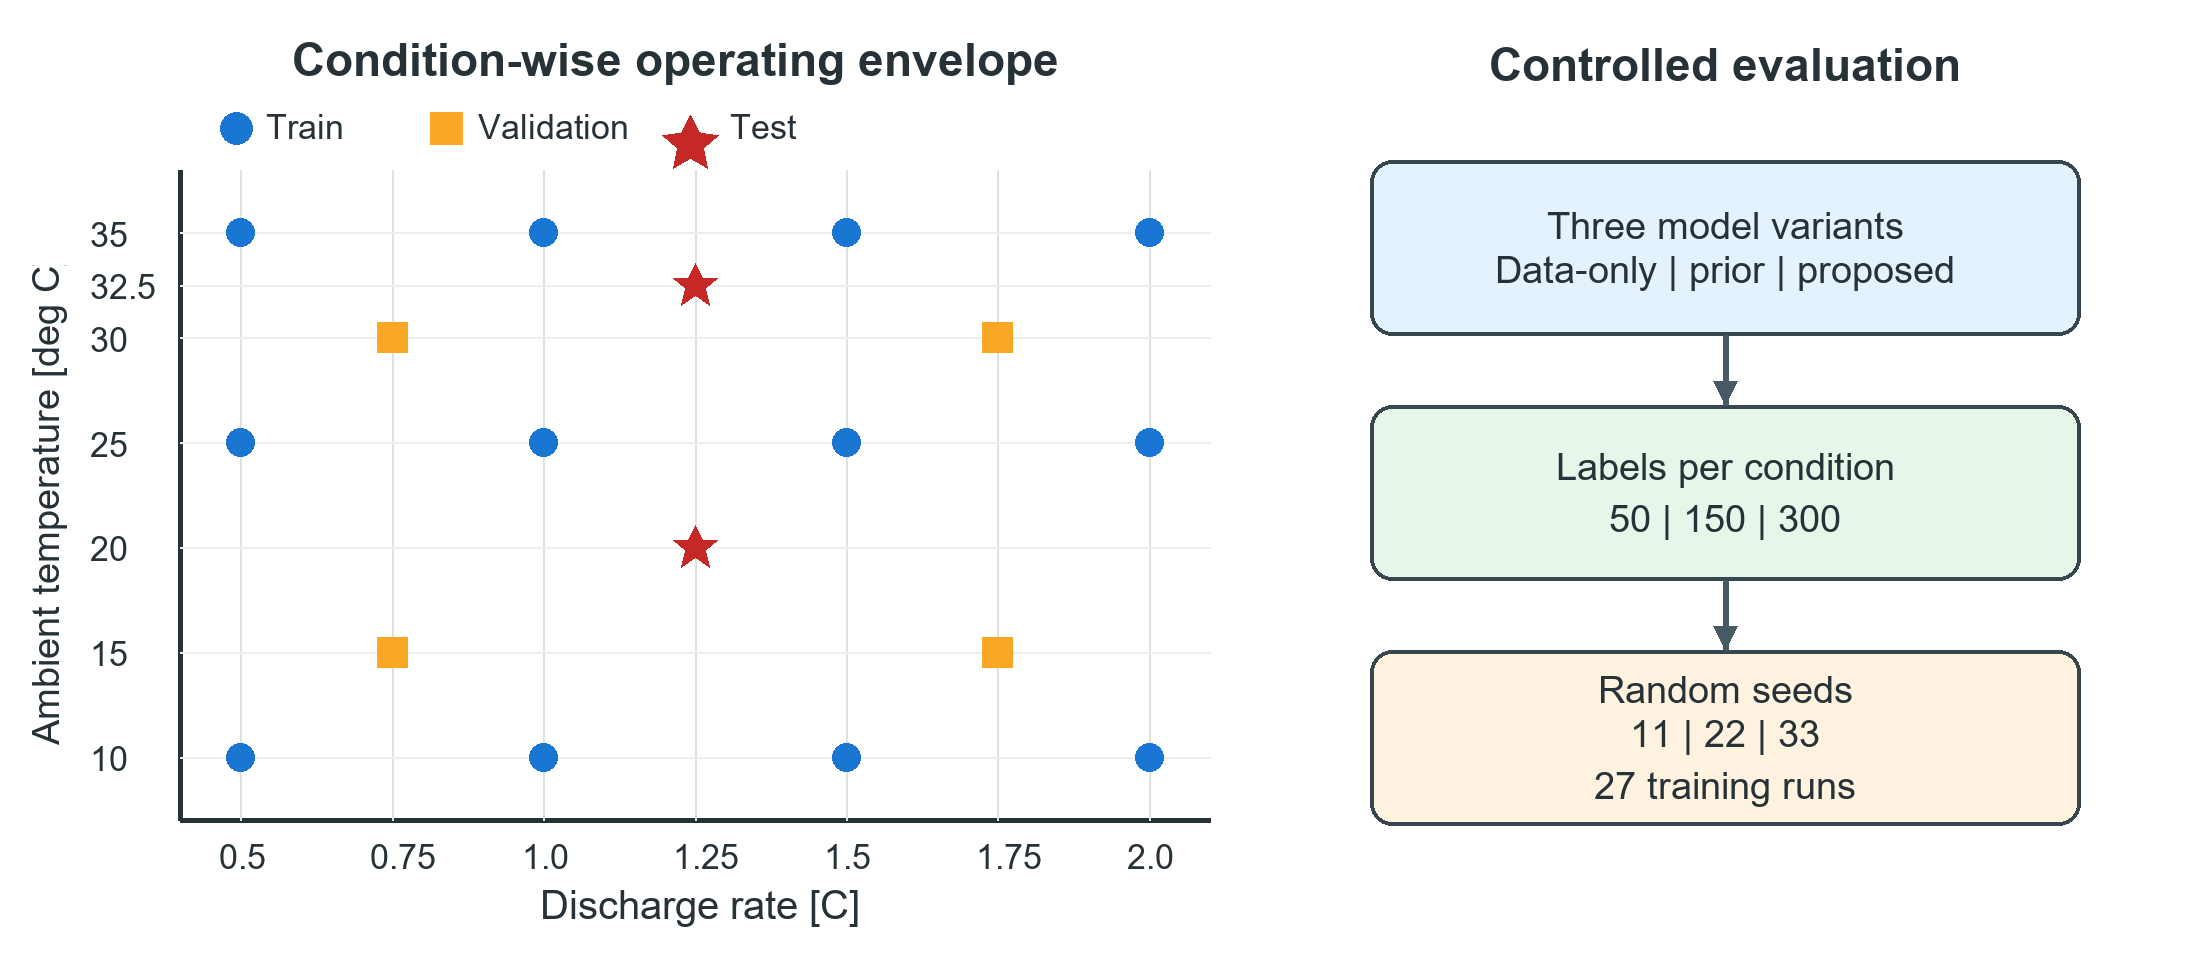
\includegraphics[width=0.96\textwidth]{experimental_design.png}
\caption{Operating-condition split and ablation protocol. Every model uses the same conditions, label budgets, and seeds.}
\label{fig:design}
\end{figure*}

\subsection{Baselines and Training Protocol}
Three variants are compared. \textbf{Data-only} uses the same four-output architecture as the earlier notebook and minimizes labeled concentration, temperature, and stress errors. \textbf{Prior-style PINN} adds diffusion, thermal, boundary, and mechanical-equilibrium residuals but retains independent stress heads. \textbf{Proposed \modelname} predicts only concentration and temperature and derives stress from concentration.

The full experiment uses label budgets of 50, 150, and 300 samples per training condition and seeds 11, 22, and 33, giving 27 runs. Adam uses a learning rate of $10^{-3}$, gradient norm clipping at 10, at most 2500 epochs, and patience of 350 epochs. Physics collocation uses 900 interior and 120 boundary samples per training condition. The selected checkpoint minimizes a validation objective and is stored before test evaluation.

\begin{table}[t]
\centering
\caption{Full Experimental Configuration}
\label{tab:config}
\footnotesize
\setlength{\tabcolsep}{3.5pt}
\begin{tabular}{p{0.43\columnwidth}p{0.50\columnwidth}}
\toprule
Item & Value \\
\midrule
Reference model & PyBaMM SPMe, lumped thermal \\
Parameter set & Chen2020 (LG M50) \\
Cutoff voltage & 2.5 V \\
Radial/time samples & 25 / 100 per condition \\
PINN hidden layers & $4\times96$, tanh \\
Optimizer & Adam, $10^{-3}$ \\
Maximum epochs / patience & 2500 / 350 \\
Interior collocation points & 900 per train condition \\
Boundary points & 120 per train condition \\
Label budgets & 50, 150, 300 \\
Random seeds & 11, 22, 33 \\
Mechanical constants & $E=15$ GPa, $\nu=0.30$ \\
Partial molar volume & $\Omega=3.497\times10^{-6}$ m$^3$ mol$^{-1}$ \\
\bottomrule
\end{tabular}
\end{table}

\subsection{Controlled Ablations}
The comparison separates two levels of change. Data-only versus prior-style PINN measures the effect of adding the available residuals while retaining the earlier four-output architecture. Prior-style PINN versus \modelname evaluates a joint redesign: replacement of the independent stress heads by the analytical concentration-to-stress map and removal of radius from the temperature branch. It cannot by itself assign an accuracy difference to only one of those changes. The three label budgets measure sample efficiency, and all budgets are reported.

Three diagnostic ablations strengthen interpretation if compute permits: remove the thermal residual while retaining temperature labels; derive stress from the data-only model's concentration; and retain the prior temperature branch while replacing only its stress heads with the analytical operator. The last comparison isolates the stress construction from the temperature-branch change. These diagnostics remain secondary to the predeclared three-model comparison.

\subsection{Evaluation Metrics}
Nine primary metrics are selected to cover predictive, physical, and computational performance. For a field $y$ with predictions $\widehat y$ over $N$ points,
\begin{align}
\operatorname{RMSE}(y)&=\sqrt{\frac{1}{N}\sum_{i=1}^{N}(\widehat y_i-y_i)^2},
\label{eq:rmse}\\
\operatorname{Rel}L_2(y)&=\frac{\|\widehat{\mathbf y}-\mathbf y\|_2}{\|\mathbf y\|_2}.
\label{eq:rell2}
\end{align}
The reported set is: (1) concentration relative $L_2$ error; (2) surface-concentration MAE; (3) temperature-rise RMSE; (4) maximum absolute temperature-rise error; (5) tangential-stress RMSE; (6) peak tensile-stress error; (7) particle mass-balance RMSE; (8) concentration--stress consistency RMSE; and (9) median inference speedup over the PyBaMM SPMe solver. Stress MAPE is excluded because stress crosses zero, making percentage errors unstable. Temperature error is measured on temperature rise rather than divided by absolute Kelvin temperature, which can hide practically relevant errors.

Independent mass conservation is checked from
\begin{equation}
\mathcal{R}_{m}=\frac{d\bar c_s}{dt}+\frac{3j_n}{FR_p},\quad
\bar c_s=\frac{3}{R_p^3}\int_0^{R_p}c_s(r,t)r^2\,dr.
\label{eq:mass}
\end{equation}
The consistency metric recomputes stress from predicted concentration and compares it with each model's reported stress. The proposed model has zero analytical inconsistency by construction, apart from floating-point and quadrature effects. For every primary metric, the paper reports mean $\pm$ standard deviation across seeds and the worst held-out condition. Improvement over the prior formulation is
\begin{equation}
\Delta_m(\%)=100\frac{m_{\mathrm{prior}}-m_{\mathrm{proposed}}}
{|m_{\mathrm{prior}}|+\epsilon},
\label{eq:gap}
\end{equation}
where positive values indicate lower proposed-model error.

\subsubsection{Inference Latency and Solver Speedup}
The ninth metric measures computational advantage. For identical held-out query batches on the same hardware, let $\widetilde t_{\mathrm{PINN}}$ and $\widetilde t_{\mathrm{SPMe}}$ be median wall-clock times over repeated blocks. The speedup is
\begin{equation}
S_{\mathrm{lat}}=\frac{\widetilde t_{\mathrm{SPMe}}}{\widetilde t_{\mathrm{PINN}}}.
\label{eq:speedup}
\end{equation}
After 100 warm-up calls, operations are synchronized and the median, 95th-percentile latency, and $S_{\mathrm{lat}}$ are reported with fixed hardware, batch size, and precision. Values above one indicate faster PINN inference. Training time is reported separately because a costly one-time fit may still yield a useful real-time surrogate.

\begin{figure}[!b]
\centering
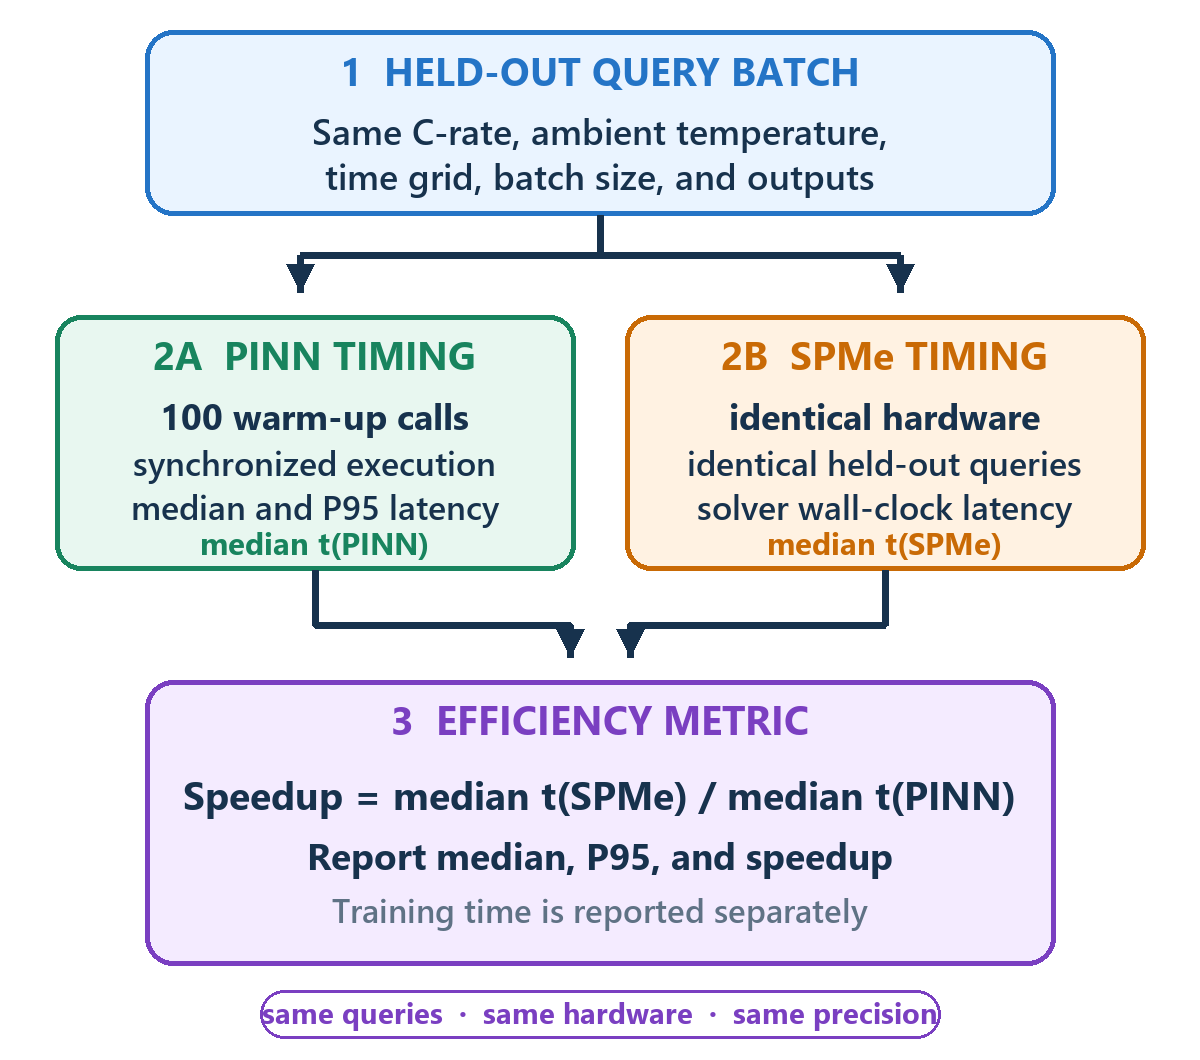
\includegraphics[width=0.98\columnwidth]{inference_efficiency_protocol_column.png}
\caption{Latency protocol using identical held-out queries and hardware, with warm-up and synchronization before PINN--SPMe comparison.}
\label{fig:latency_protocol}
\end{figure}

\subsection{Statistical Summary and Acceptance Criteria}
For each model--budget pair, metrics are evaluated separately for the two test conditions and three seeds. The primary summary is the seed mean and sample standard deviation after averaging the two conditions within each seed. The worst-condition column is retained because an apparently strong mean can conceal failure at one ambient temperature. Since only three seeds are used, the standard deviation is descriptive; it should not be presented as proof of statistical significance.

A result supports the central hypothesis only when three conditions hold together: the proposed model reduces concentration--stress inconsistency as designed, its stress RMSE or peak-stress error does not materially worsen, and its concentration and temperature errors remain competitive over the label budgets. A zero consistency residual alone is a property of the architecture, not evidence of predictive accuracy. Inference latency is accepted only when the protocol in Fig.~\ref{fig:latency_protocol} is followed; training time and parameter count remain secondary resource measures.

\section{Results and Discussion}
\subsection{Result-Reporting Contract}
Table~\ref{tab:results} is connected conceptually to the notebook outputs \texttt{paper\_metrics\_summary.csv} and \texttt{variation\_gap\_vs\_previous.csv}. The manuscript intentionally does not insert guessed values. Before submission, the full configuration must be run with \texttt{quick\_mode=False}; the result macros at the beginning of this file must then be replaced with the reported mean $\pm$ standard deviation. This preserves a strict boundary between a reproducible methodology and empirical claims.

\begin{table*}[t]
\centering
\caption{Held-Out Test Performance at 300 Labels per Training Condition (Mean $\pm$ Standard Deviation Across Three Seeds)}
\label{tab:results}
\footnotesize
\resizebox{0.98\textwidth}{!}{%
\begin{tabular}{lccccc}
\toprule
Model & Concentration Rel-$L_2$ & Temp.-rise RMSE [K] & Tangential-stress RMSE [MPa] & Mass-balance RMSE [mol m$^{-3}$ s$^{-1}$] & Median speedup [$\times$] \\
\midrule
Data-only & \DataC & \DataT & \DataStress & \DataMass & \DataSpeed \\
Prior-style PINN & \PriorC & \PriorT & \PriorStress & \PriorMass & \PriorSpeed \\
Proposed \modelname & \ProposedC & \ProposedT & \ProposedStress & \ProposedMass & \ProposedSpeed \\
\bottomrule
\end{tabular}
}
\end{table*}

\subsection{Required Plots and Traceability}
Four plots are generated from saved CSV files: error versus label budget, predicted and reference surface concentration, temperature rise, and radial/tangential stress profiles. Each identifies the held-out condition and summarizes all seeds. A fifth plot shows mass-balance residual. Aggregate metrics measure overall performance; trajectories expose phase, boundary, and localized peak-stress errors hidden by one scalar.

All tables and plots use the same per-condition file. The aggregation script verifies 27 planned runs, partition separation, and three distinct seeds per mean. Failed runs are marked incomplete rather than silently averaged over fewer seeds.

\subsection{Questions the Experiment Must Resolve}
The evaluation asks whether physics constraints reduce sparse-label error and whether analytical concentration--stress coupling improves mechanical credibility without degrading concentration or temperature accuracy. Evidence requires consistent multi-seed behavior, peak-stress and stress-RMSE checks, conservation results, and worst-condition reporting. Held-out conditions test interpolation inside the sampled C-rate and temperature envelope; they do not establish extrapolation to charging, drive cycles, extreme temperatures, or unseen chemistries.

\subsection{Physical Interpretation and Prior Work}
During discharge, a surface-to-core concentration gradient produces diffusion-induced stress, while uniform concentration gives zero stress; higher rates should increase transient nonuniformity. Temperature rise follows heat generation and convective loss in Eq.~\eqref{eq:thermal}. Unlike parameter-inference surrogates \cite{hassanaly2024part1,hassanaly2024part2}, aging-informed SOH models \cite{wei2026etm}, and life-cycle temperature predictors \cite{wang2023temperature}, this study tests analytical mechanical consistency during discharge. These expectations guide interpretation but do not replace measured errors.

\section{Limitations and Threats to Validity}
All labels are simulated. PyBaMM is a credible and reproducible reference environment, but agreement with an SPMe simulation is not experimental validation. The model uses a negative-electrode representative particle, lumped cell temperature, prescribed material parameters, and constant-current discharge. It does not represent through-cell temperature gradients, heterogeneous electrode stress, plasticity, binder effects, fracture initiation, or feedback from stress to diffusion.

The mechanical constants are assumed rather than calibrated to the particular LG M50 cell. Consequently, stress results are best interpreted as analytical diffusion-induced stress indicators. The Chen2020 parameter set was developed from multiscale experiments, yet PyBaMM documentation cautions that parameter sets are model inputs rather than certificates of a cell's true internal properties \cite{chen2020parameterization}. Material sensitivity analysis is recommended before making quantitative mechanical claims.

The heat-generation history in the training references is obtained from the SPMe simulation. The resulting model learns a parameterized mapping over the sampled constant-current envelope; it has not been shown to accept arbitrary current profiles. Additionally, PINN optimization can suffer from competing gradient scales. Multiple seeds and independent residual checks reduce the risk of reporting a favorable but unstable checkpoint, but they do not eliminate model-form error.

No degradation claim is supported. Adding SEI growth, lithium plating, loss of active material, or crack propagation is scientifically possible in PyBaMM \cite{sulzer2021pybamm}; however, a defensible aging study also requires cycling protocols, capacity or health targets, degradation parameters, and held-out cells or profiles. Mechanical state and degradation can coexist, but one should not be substituted for the other merely to increase the number of equations.

\subsection{Parameter Sensitivity and Uncertainty}
Stress scales with $E\Omega/(1-\nu)$ in Eqs.~\eqref{eq:sr} and \eqref{eq:st}, so uncertain material constants can dominate stress error even when concentration is accurate. The sensitivity study passes each saved concentration prediction through the analytical operator while varying $E$ and $\Omega$ independently by $\pm20\%$; it reports the corresponding peak-stress change without retraining. Because $D_s$ is fixed during training, conclusions remain restricted to Chen2020 rather than changing diffusivity after fitting.

Quadrature uncertainty is checked at 25, 50, and 100 radial points. Peak stress and mass-balance error must stabilize with refinement, separating numerical integration error from a genuine physics violation.

\subsection{Failure Analysis Protocol}
Failures are separated into data, physics, and coupling errors. Large concentration error with a small residual points to boundary, initialization, or scaling error; small data error with a large residual indicates unreliable off-grid physics. Accurate concentration with poor stress implicates material constants or quadrature. A temperature offset suggests heat-generation or heat-capacity error, whereas ambient-dependent growth suggests cooling mismatch.

Non-finite runs, implausibly early checkpoints, and runs still improving at the epoch limit are flagged from validation and residual histories; their causes and counts are reported without replacing difficult seeds. The held-out conditions test interpolation only. Claims of robustness require additional noise, parameter shifts, or current-profile tests, and a low residual establishes agreement with the imposed equations rather than completeness of the physics.

\balance
\section{Conclusion}
This paper defines an electrochemical--thermal PINN with particle stress derived analytically from predicted concentration. It also uses lumped thermal physics, fixed physical-time normalization, condition-wise splits, validation-only checkpointing, and controlled sparse-label evaluation. The contribution is this cross-field construction and its evaluation protocol, not a claim that electrochemical--thermal--mechanical modeling is new.

The empirical conclusion must use the complete three-seed run. Lower stress error and label sensitivity with retained concentration and temperature accuracy would support structural physics coupling. If only consistency improves, the result instead motivates better concentration training, adaptive loss balancing, or calibrated material parameters. Future work will add experiments, dynamic currents, uncertainty analysis, and degradation with appropriate cycling data.

\section*{Data and Code Availability}
The accompanying Colab notebook generates PyBaMM data, trains all baselines, and exports metrics, checkpoints, and the label-budget ablation. Data and weights should be archived with the software versions and seeds in Table~\ref{tab:config}.

\section*{Acknowledgment}
The authors acknowledge the Department of Computer Science and Engineering, KPR Institute of Engineering and Technology, for supporting this project.

\begin{thebibliography}{00}
\setlength{\itemsep}{0pt}
\bibitem{doyle1993dfn}
M. Doyle, T. F. Fuller, and J. Newman, ``Modeling of galvanostatic charge and discharge of the lithium/polymer/insertion cell,'' \emph{J. Electrochem. Soc.}, vol. 140, no. 6, pp. 1526--1533, 1993, doi: 10.1149/1.2221597.

\bibitem{marquis2019spme}
S. G. Marquis, V. Sulzer, R. Timms, C. P. Please, and S. J. Chapman, ``An asymptotic derivation of a single particle model with electrolyte,'' \emph{J. Electrochem. Soc.}, vol. 166, no. 15, pp. A3693--A3706, 2019, doi: 10.1149/2.0341915jes.

\bibitem{richardson2020gspm}
G. Richardson, I. Korotkin, R. Ranom, M. J. Castle, and J. M. Foster, ``Generalised single particle models for high-rate operation of graded lithium-ion electrodes: Systematic derivation and validation,'' \emph{Electrochim. Acta}, vol. 339, art. 135862, 2020, doi: 10.1016/j.electacta.2020.135862.

\bibitem{planella2022continuum}
F. Brosa Planella \emph{et al.}, ``A continuum of physics-based lithium-ion battery models reviewed,'' \emph{Prog. Energy}, vol. 4, no. 4, art. 042003, 2022, doi: 10.1088/2516-1083/ac7d31.

\bibitem{raissi2019pinn}
M. Raissi, P. Perdikaris, and G. E. Karniadakis, ``Physics-informed neural networks: A deep learning framework for solving forward and inverse problems involving nonlinear partial differential equations,'' \emph{J. Comput. Phys.}, vol. 378, pp. 686--707, 2019, doi: 10.1016/j.jcp.2018.10.045.

\bibitem{hassanaly2024part1}
M. Hassanaly \emph{et al.}, ``PINN surrogate of Li-ion battery models for parameter inference, Part I: Implementation and multi-fidelity hierarchies for the single-particle model,'' \emph{J. Energy Storage}, vol. 98, art. 113103, 2024, doi: 10.1016/j.est.2024.113103.

\bibitem{hassanaly2024part2}
M. Hassanaly \emph{et al.}, ``PINN surrogate of Li-ion battery models for parameter inference, Part II: Regularization and application of the pseudo-2D model,'' \emph{J. Energy Storage}, vol. 98, art. 113104, 2024, doi: 10.1016/j.est.2024.113104.

\bibitem{wang2023temperature}
Y. Wang, C. Xiong, Y. Wang, P. Xu, C. Ju, J. Shi, G. Yang, and J. Chu, ``Temperature state prediction for lithium-ion batteries based on improved physics informed neural networks,'' \emph{J. Energy Storage}, vol. 73, art. 108863, 2023, doi: 10.1016/j.est.2023.108863.

\bibitem{wang2024parameter}
J. Wang, Q. Peng, J. Meng, T. Liu, J. Peng, and R. Teodorescu, ``A physics-informed neural network approach to parameter estimation of lithium-ion battery electrochemical model,'' \emph{J. Power Sources}, vol. 621, art. 235271, 2024, doi: 10.1016/j.jpowsour.2024.235271.

\bibitem{wei2026etm}
Y. Wei, K. Liu, J. Rui, and Q. Zhao, ``Integrating electrochemical-thermal-mechanical physical informed neural network framework for lithium-ion batteries state of health estimation,'' \emph{Energy AI}, vol. 24, art. 100713, 2026, doi: 10.1016/j.egyai.2026.100713.

\bibitem{cheng2009stress}
Y.-T. Cheng and M. W. Verbrugge, ``Evolution of stress within a spherical insertion electrode particle under potentiostatic and galvanostatic operation,'' \emph{J. Power Sources}, vol. 190, no. 2, pp. 453--460, 2009, doi: 10.1016/j.jpowsour.2009.01.021.

\bibitem{zhuang2026spm}
Y. Zhuang, Y. Zheng, Y. Che, and R. Teodorescu, ``Physics-informed neural network surrogate modeling of single particle model for lithium-ion batteries,'' arXiv:2601.01466, 2026.

\bibitem{fu2024spacecraft}
H. Fu, Z. Liu, K. Cui, Q. Du, J. Wang, and D. Shi, ``Physics-informed neural network for spacecraft lithium-ion battery modeling and health diagnosis,'' \emph{IEEE/ASME Trans. Mechatronics}, vol. 29, no. 5, pp. 3546--3555, 2024, doi: 10.1109/TMECH.2023.3348519.

\bibitem{dang2024soc}
L. Dang, J. Yang, M. Liu, and B. D. Chen, ``Differential equation-informed neural networks for state-of-charge estimation,'' \emph{IEEE Trans. Instrum. Meas.}, vol. 73, pp. 1--12, 2024, doi: 10.1109/TIM.2023.3334377.

\bibitem{ye2024soh}
J. Ye, Q. Xie, M. Lin, and J. Wu, ``A method for estimating the state of health of lithium-ion batteries based on physics-informed neural network,'' \emph{Energy}, vol. 294, art. 130828, 2024, doi: 10.1016/j.energy.2024.130828.

\bibitem{jiang2025heatmap}
Y. Jiang, Z. Liu, P. Kabirzadeh, Y. Wu, Y. Li, N. Miljkovic, and P. Wang, ``Multi-fidelity physics-informed convolutional neural network for heat map prediction of battery packs,'' \emph{Reliab. Eng. Syst. Saf.}, vol. 256, art. 110752, 2025, doi: 10.1016/j.ress.2024.110752.

\bibitem{tian2025generic}
A. Tian, L. He, T. Ding, K. Dong, Y. Wang, and J. Jiang, ``A generic physics-informed neural network framework for lithium-ion batteries state of health estimation,'' \emph{Energy}, vol. 332, art. 137215, 2025, doi: 10.1016/j.energy.2025.137215.

\bibitem{xiong2025diagnostics}
R. Xiong, Y. He, Y. Sun, Y. Jia, and W. Shen, ``Enhanced electrode-level diagnostics for lithium-ion battery degradation using physics-informed neural networks,'' \emph{J. Energy Chem.}, vol. 104, pp. 618--627, 2025, doi: 10.1016/j.jechem.2025.01.019.

\bibitem{chen2025smallsample}
L. Chen \emph{et al.}, ``Physics-informed neural networks for small sample state of health estimation of lithium-ion batteries,'' \emph{J. Energy Storage}, vol. 122, art. 116559, 2025, doi: 10.1016/j.est.2025.116559.

\bibitem{luo2025hybrid}
Y. Luo, S. Ju, P. Li, and H. Zhang, ``A method for estimating lithium-ion battery state of health based on physics-informed hybrid neural network,'' \emph{Electrochim. Acta}, vol. 525, art. 146110, 2025, doi: 10.1016/j.electacta.2025.146110.

\bibitem{lyu2024digitaltwin}
C. Lyu, S. Xu, J. Li, and M. Pecht, ``Digital twin modeling method for lithium-ion batteries based on data-mechanism fusion driving,'' \emph{Green Energy Intell. Transp.}, vol. 3, no. 5, art. 100162, 2024, doi: 10.1016/j.geits.2024.100162.

\bibitem{christensen2006fracture}
J. Christensen and J. Newman, ``A mathematical model of stress generation and fracture in lithium manganese oxide,'' \emph{J. Electrochem. Soc.}, vol. 153, no. 6, pp. A1019--A1030, 2006, doi: 10.1149/1.2185287.

\bibitem{xu2016electrochemomechanics}
R. Xu and K. Zhao, ``Electrochemomechanics of electrodes in Li-ion batteries: A review,'' \emph{J. Electrochem. Energy Convers. Storage}, vol. 13, no. 3, art. 030803, 2016, doi: 10.1115/1.4035310.

\bibitem{sulzer2021pybamm}
V. Sulzer, S. G. Marquis, R. Timms, M. Robinson, and S. J. Chapman, ``Python Battery Mathematical Modelling (PyBaMM),'' \emph{J. Open Res. Softw.}, vol. 9, no. 1, art. 14, 2021, doi: 10.5334/jors.309.

\bibitem{chen2020parameterization}
C.-H. Chen, F. Brosa Planella, K. O'Regan, D. Gastol, W. D. Widanage, and E. Kendrick, ``Development of experimental techniques for parameterization of multi-scale lithium-ion battery models,'' \emph{J. Electrochem. Soc.}, vol. 167, no. 8, art. 080534, 2020, doi: 10.1149/1945-7111/ab9050.

\bibitem{bernardi1985energy}
D. Bernardi, E. Pawlikowski, and J. Newman, ``A general energy balance for battery systems,'' \emph{J. Electrochem. Soc.}, vol. 132, no. 1, pp. 5--12, 1985, doi: 10.1149/1.2113792.

\end{thebibliography}

\end{document}


